\section{Plan, forecast and recurrence records}
\label{app:temporal}

The exhibits below are inherited from the baseline temporal extension, whose quoted excerpts were source-checked against the original fields (\path{agenda_longitudinal_witnesses.json}). The 240-record sample is described in Section~\ref{sec:temporal}.

\begin{table}[htbp]
\centering\small
\begin{tabularx}{\linewidth}{@{}llX@{}}
\toprule
Decision & Turn & Stated target or applied step (G9, Sol)\\
\midrule
d64 & 29 & Ends with \$27 and the target of three houses on each dark blue as funds arrive.\\
d65--67 & 30 & Buys Vermont, mortgages Pennsylvania Railroad, adds one Boardwalk house; \$27 remains.\\
d102 & 39 & Adds one Park Place house; \$167 remains.\\
d162--163 & 60 & Mortgages Connecticut, then adds one house to each dark blue.\\
d164 & 60 & Both properties have three houses; cash is \$17.\\
\bottomrule
\end{tabularx}
\caption{A recorded development target realized over 31 turns. The rows are milestones; financing, trades and movement intervene. Target attainment does not show a causal benefit of memory or an optimal investment.}
\label{tab:g9}
\end{table}

\begin{table}[htbp]
\centering\small
\begin{tabularx}{\linewidth}{@{}p{0.24\linewidth}X@{}}
\toprule
Record & Evidence (G16)\\
\midrule
Grok, d103, applied note & ``End, buy Virginia on sight, then house pink''\\
Actual d159 menu & Virginia purchase offered for \$160; Grok has \$371.\\
Grok, d159, applied note & ``Buy at list is the only way to close pink.''\\
Grok, d159, applied action & \texttt{start\_auction}; the public message says ``Virginia is mine. Pink set closed.''\\
Gemini, d162 & Bids \$380.\\
After d164 & Virginia assigned to Gemini for \$380 (event 1277).\\
\bottomrule
\end{tabularx}
\caption{A stated purchase plan meets an affordable legal opportunity, and the applied action contradicts the same response's note. Of eight sampled explicit landing-purchase policies, six meet no later opportunity, one is executed and this one is not. These outcomes are not a planning score.}
\label{tab:g16}
\end{table}

\begin{table}[htbp]
\centering\small
\begin{tabularx}{\linewidth}{@{}llX@{}}
\toprule
Game & Decision & Stated rule and applied bid (Grok)\\
\midrule
G20 & d40 & Bids \$228; note says to drop at \$236 or above.\\
 & d42 & Bids \$230 and tightens the rule: ``do not chase past \$230.''\\
 & d44 & Bids \$232: ``Prior note said drop at \$231+, but \$232 is only \$2 past the hard stop''.\\
 & d46 & Drops when the next minimum is \$234; the original \$235 bound is not exceeded.\\
\midrule
G17 & d228 & Cash is \$99; note says ``Do not drop before \$99.''\\
 & d230--231 & Bids \$40; the rival jumps to \$100.\\
 & d232 & Drops because the next minimum, \$101, exceeds its cash, as its ceiling implied.\\
\bottomrule
\end{tabularx}
\caption{A revised limit and a respected limit. G20 shows a stated rule revised within one auction; G17 is a control against coding every withdrawal below a nominal cap as inconsistent.}
\label{tab:auctions}
\end{table}

\begin{table}[htbp]
\centering\small
\begin{tabularx}{\linewidth}{Yrrr}
\toprule
Episode population & Episodes & Later submission & Error repeated\\
\midrule
All uneven-error decisions & 114 & 109 & 63\\
Exact error in a later corrective request & 54 & 50 & 9\\
First such request per player-game & 31 & 29 & 2\\
\bottomrule
\end{tabularx}
\caption{Construction-error recurrence at the next distinct decision with a submitted build. Populations overlap, and missing later submissions are censored rather than counted as repairs. Forty-eight of the 54 feedback episodes end in some applied build; four of the 44 with a later submission repeat the error, against five of the six without an applied build.}
\label{tab:recurrence}
\end{table}

\begin{figure}[htbp]
\centering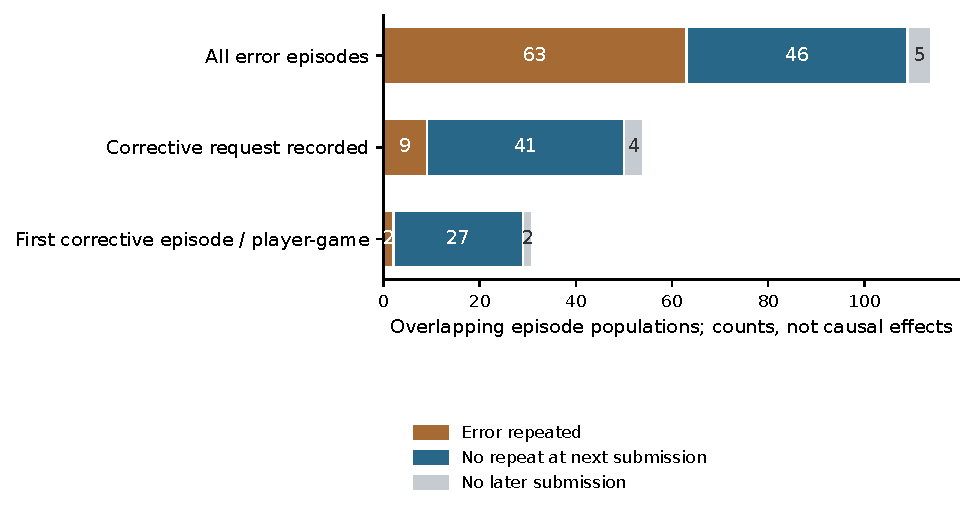
\includegraphics[width=0.78\linewidth]{error_recurrence.pdf}
\caption{The same three overlapping episode populations as Table~\ref{tab:recurrence}. Counts, not effects of feedback.}
\label{fig:recurrence}
\end{figure}

At G17 d228 Grok also predicts that a rival will outbid its \$99 ceiling and still build. The rival outbids, but jail, a fine and debt liquidation follow before its first management decision at d257 with \$63, and no later menu offers construction before its elimination at d267. The forecast is neither confirmed nor falsified by this record.
